% #############################################################################
% This is Chapter 4
% !TEX root = ../main.tex
% #############################################################################
% Change the Name of the Chapter i the following line
\fancychapter{Algorithmic Optimization in Architecture}
%\cleardoublepage
% The following line allows to ref this chapter
\label{chap:implement}
In the previous chapter, we discussed the architecture of the proposed solution, a general-purpose optimization framework that is applicable to a wide variety of optimization problems. 

From the beginning, we set out to address optimization problems involving simulation-based objective functions that are remarkably expensive. Therefore, during the development of the proposed framework, we focused on providing algorithms to more efficiently handle problems exhibiting these properties. Note, however, that the framework can be easily extended to include other algorithms (e.g., derivative-based), as it has been previously discussed in \cref{sec:optalgos}. 

Motivated by the large impact of the building sector in the world's sustainability and economy, this dissertation aims at applying the proposed framework to address \ac{BPO} problems, thus attempting to reduce buildings sector' costs and ecological footprints. Despite the existence of multiple optimization tools in architecture, as discussed in \cref{sec:optimizationtools}, these are often limited and do not provide adequate algorithms, nor mechanisms to enable the efficient optimization of such time-consuming problems.

In this chapter, we describe how the general-purpose framework proposed in this dissertation can be applied to address architectural design optimization. 

\section{Algorithmic Optimization}
In \cref{ssec:ad,ssec:aa}, we discussed how the architectural design paradigm has incrementally grown to develop the mechanisms to quickly (1) update a design, (2) generate the corresponding analytical model, and (3) automatically evaluate the design in an analytical tool.% and collect its results. 

These mechanisms laid down the foundations for automated optimization processes. By extending the Algorithmic Design and Analysis (\ac{ADA}) approach to include optimization mechanisms, we are able to apply automatic optimization processes that aim to improve (or even optimize) designs' performance. 

\Cref{fig:algorithmicoptimization} illustrates a possible approach for introducing automated optimization processes in the architectural worfklow. In this approach, we introduce an optimizer component that is responsible for searching the design space and generating new values for the design's parameters. These values are then communicated to the \ac{AD} tool, which generates the analytical models and evaluates them in the corresponding analytical tools. After being evaluated, the analytical tools communicate the evaluations' results to the \ac{AD} tool, which, in turn, forwards them to the optimizer. Based on these results, the optimizer generates another set of values for the design's parameters and this process is repeated until a stopping criterion (e.g., evaluations or time limit, solution's quality) is met. The communications between each component are encoded within the \ac{AD} tool, therefore incurring no additional efforts for the architect.
 
 \begin{figure}[htbp]
 	\centering
 	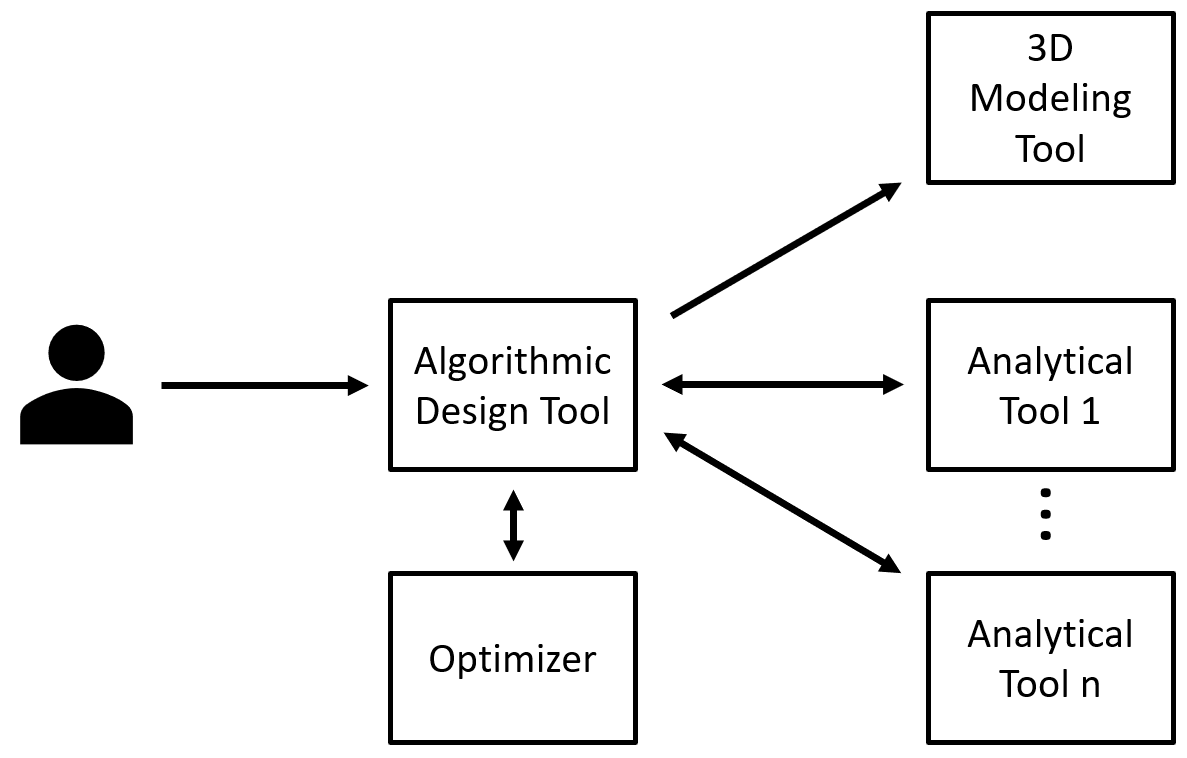
\includegraphics[width=0.6\textwidth]{./Images/Solution/algorithmic_optimization.png}
 	\caption[Algorithmic Optimization workflow]{Algorithmic Optimization workflow. In this workflow, the architect only interacts with an \ac{AD} tool to create the initial design, to specify the analysis tools, and to specify the optimization parameters.}
 	\label{fig:algorithmicoptimization}
 \end{figure}
 
In order to benefit from this approach, which we name \ac{AO}, we combine the optimization framework developed in this dissertation with an \ac{AD} tool to provide an alternative to easily address a wide variety of \ac{BPO} problems. To this end, architects are required to: (1) create the \ac{AD} model reflecting their design's intents; (2) select the performance aspects to optimize and, thus, the analysis tools to be used (e.g., lighting, thermal, structural, costs), and, finally, (3) select, if necessary, the parameters of the optimization process (e.g., algorithm, algorithm's parameters). %In the end, architects are only required to run the script and the optimization process will automatically start. 
\Cref{BPOjuliaCode} presents a simple example of an \ac{AO} approach using the developed framework and the Khepri \ac{AD} tool, where the architect: (1) defines the algorithmic description of the intended design (\textit{lines 1-4}), (2) defines four variables and their acceptable variation range (\textit{lines 17-20}), (3) defines the objective functions for the performance aspects to consider in the optimization (\textit{lines 6-14 and 21-22}), (4) creates the optimization model (\textit{line 23}), (5) defines the algorithm's parameters (\textit{line 24}), and (6) specifies the optimization algorithm and the maximum number of evaluations (\textit{line 25}).

Even though the provided example presents a textual-based \ac{AO} approach, the developed optimization framework can easily be integrated within a visual \ac{AD} tool, like Grasshopper. 

One important aspect that results from this combination is the fact that architects are able to use different optimization algorithms and, consequently, to select an optimization algorithm that better suits their problems. To bridge the gap between the lack of knowledge or experience and the suitability of optimization algorithms for each problem, the optimization framework also provides automated testing mechanisms. These mechanisms enable the sequential execution of multiple optimization algorithms for a specified amount of evaluations, as well as each algorithm's performance measures. This feature is particularly important in the architectural context~\cite{Wortmann2016BBO,Hamdy2016}, as it promotes more informed decisions towards the selection of more appropriate optimization algorithms.

\begin{lstlisting}[caption={BPO example of the framework's API using the Khepri AD tool},label=BPOjuliaCode]	
building_with_skylight(height, width, length, material) = let
	# Create the design using Khepri's primitives
	...
end

# Analytical-based criterium
cost(height, width, length, material) = let
	p1 = width * length * 185,
	p2 = (width + length) * 2 * height * 80
	p1 + p2
end

# Simulation-based criterium
daylight(height, width, length, material) = radiance_analysis(...)

# Optimization Process
let height = RealVariable(0.1, 2),
	width = RealVariable(0.1, 6.5),
	length = RealVariable(0.1, 11),
	material = IntVariable(0, 3),
	obj1 = Objective(daylight, :MAX),
	obj2 = Objective(cost, :MIN),
	model = Model([height, width, length, material], [obj1, obj2]),
	NSGA_params = Dict(:population_size => 10)
  solve(NSGAII, NSGA_params, model, max_evals=100)
end
\end{lstlisting}

Due to the visual nature of architects and the generalized lack of confidence in optimization processes, the visualization of evaluated design solutions is of great importance, as it allows architects to explore and corroborate the optimization results. To this end, the optimization framework provides post-processing and visual mechanisms (see \cref{fig:postprocessing}) that, when combined with an \ac{AD} tool, allow the architect to click on the evaluated solutions and instantly visualize the corresponding design in a 3D modeling tool. 

\begin{figure*}[htbp]
	\centering
	\subfigure[]{%
		\label{fig:postprocessing-a}%
		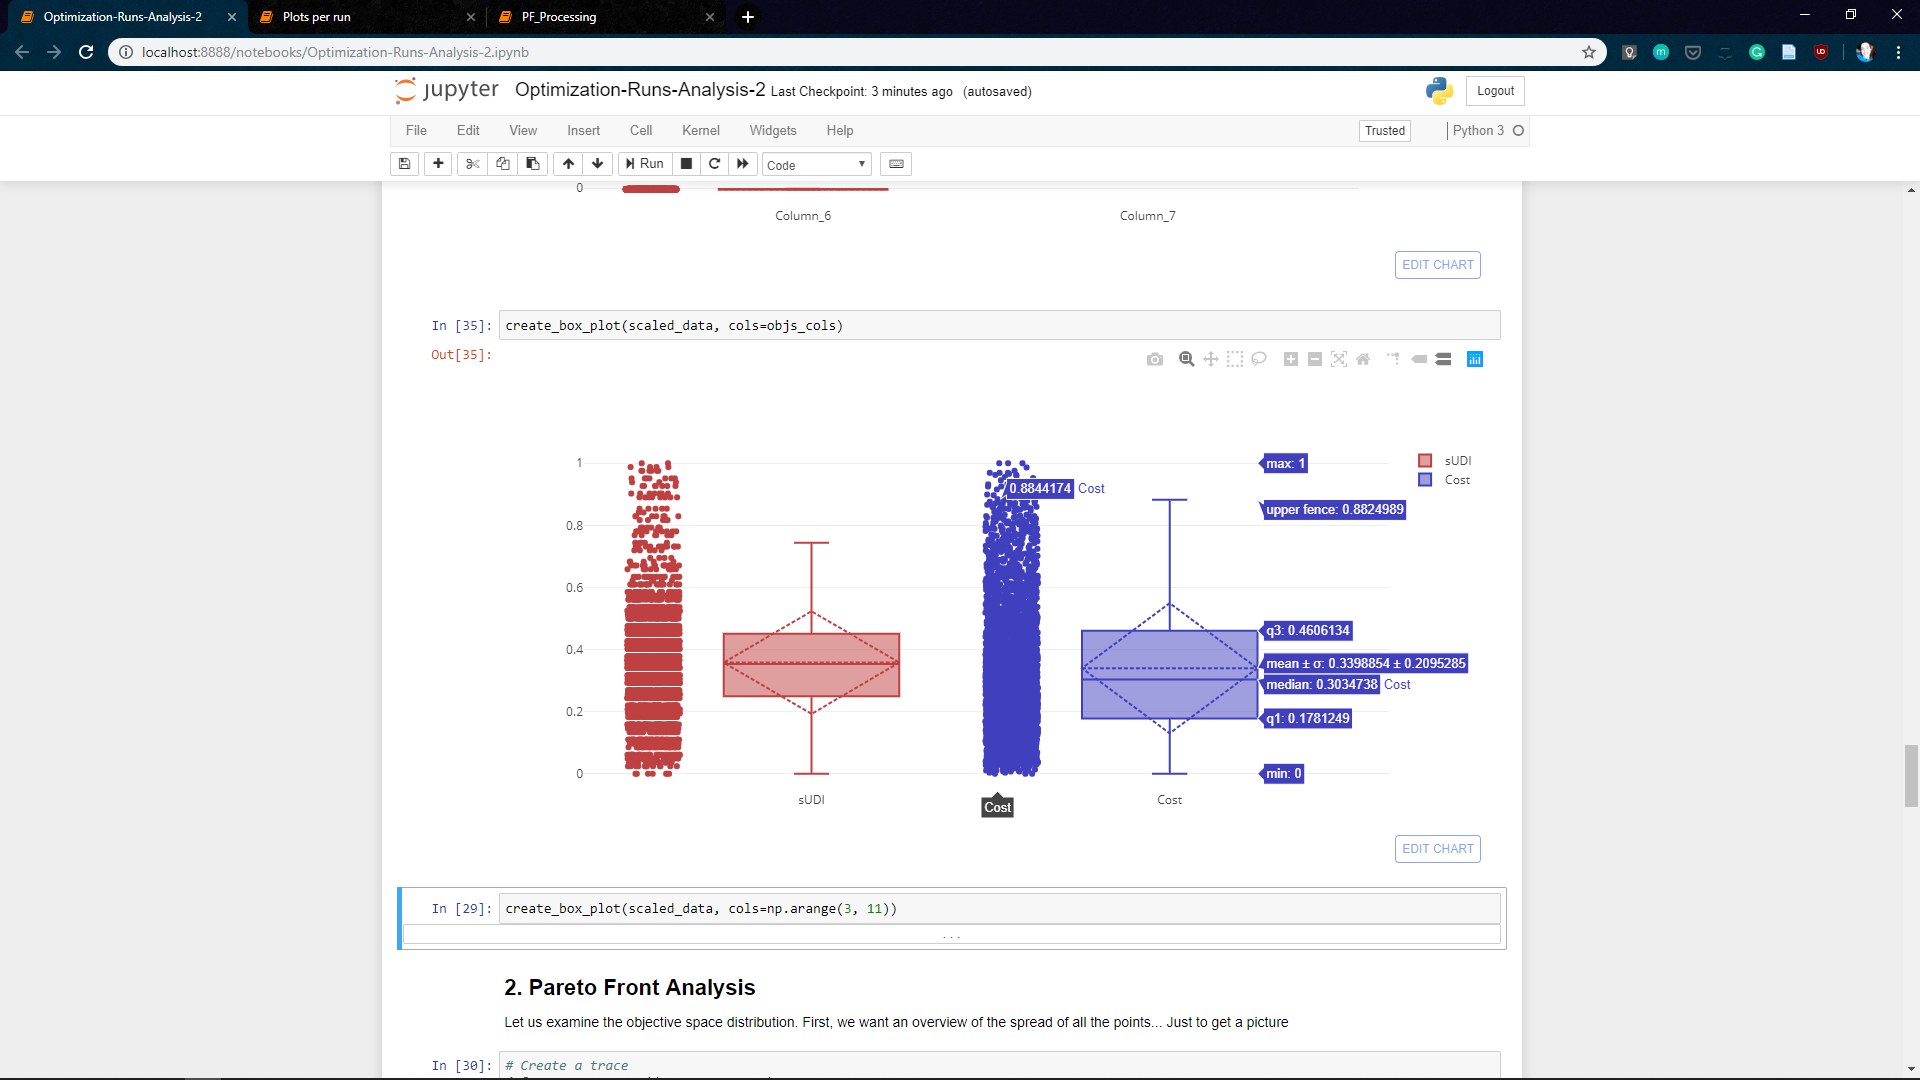
\includegraphics[width=0.485\textwidth]{./Images/Solution/postprocessing.png}}%
	\hfill
	\subfigure[]{%
		\label{fig:postprocessing-b}%
		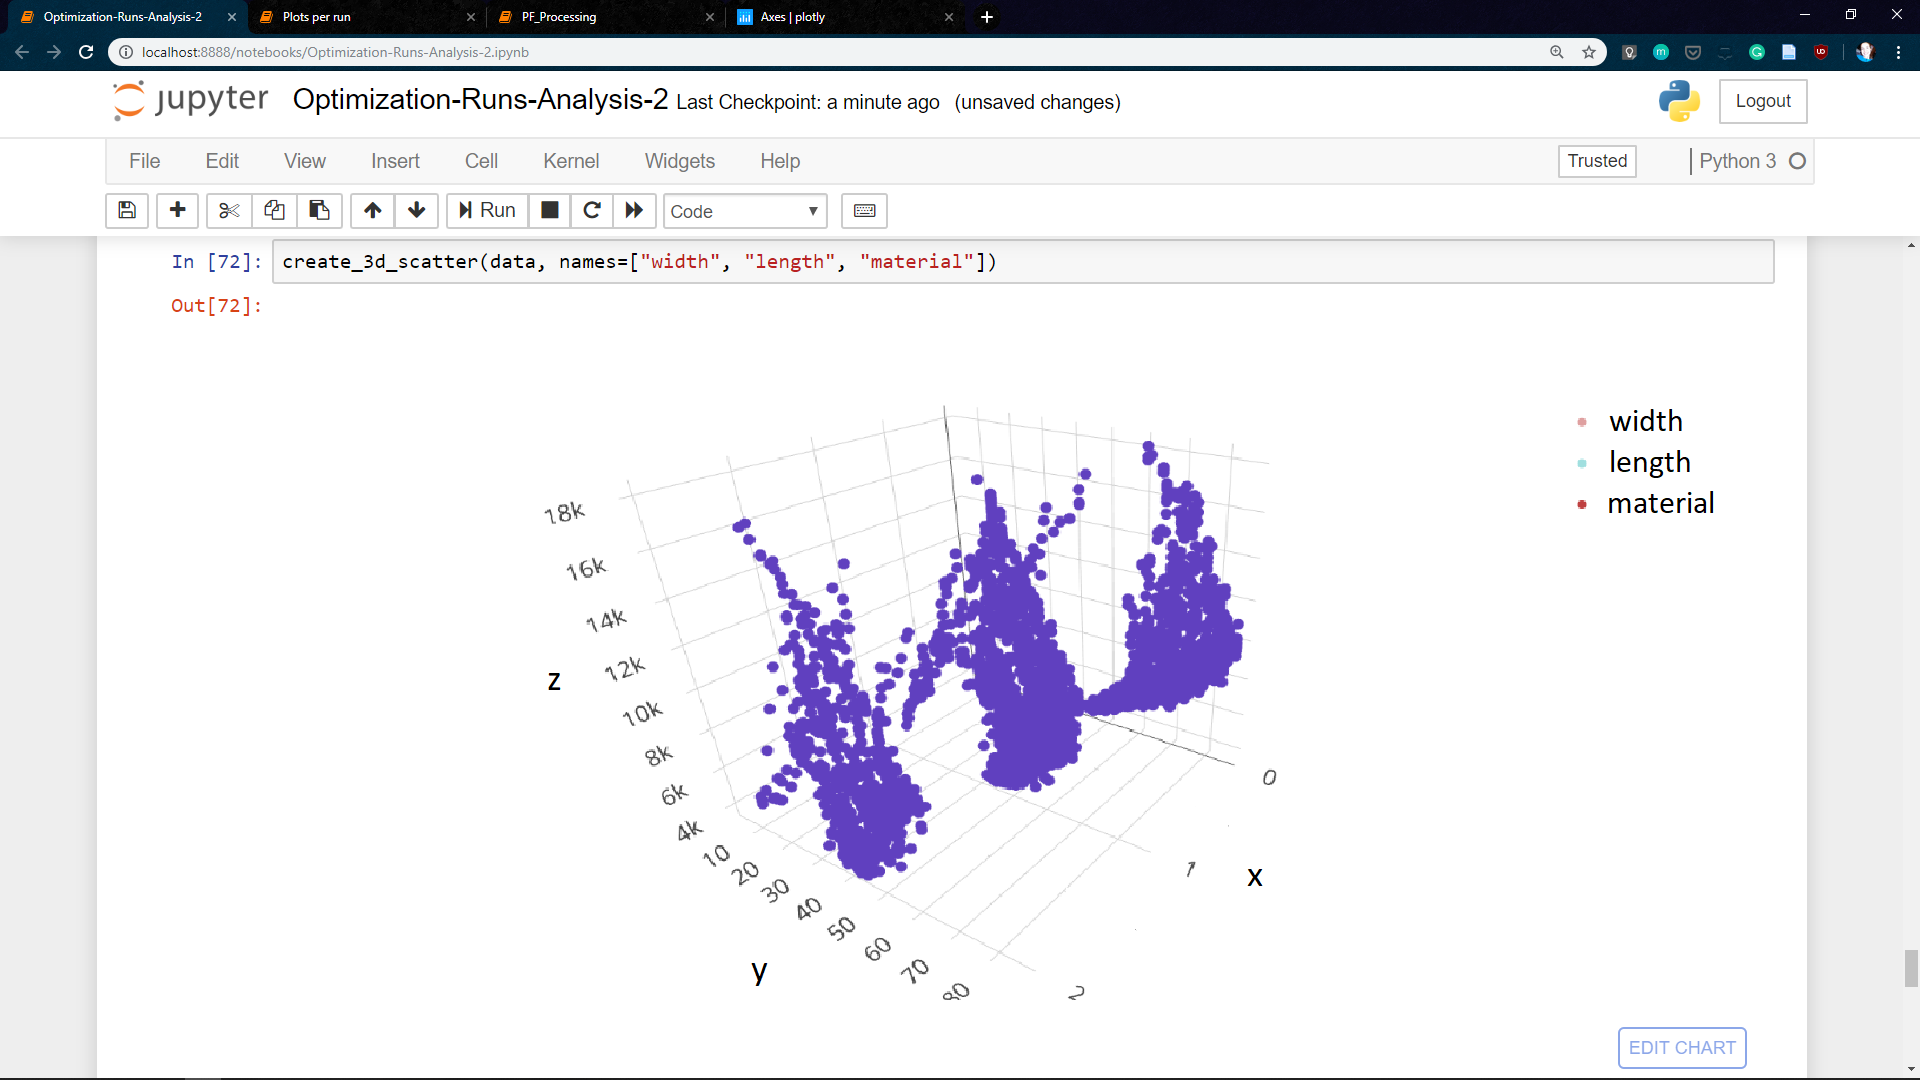
\includegraphics[width=0.485\textwidth]{./Images/Solution/postprocessing3-Copy.png}}%
	
	\caption[Examples of the post processing and visual mechanisms of the proposed solution]{Examples of the post processing and visual mechanisms (a) Box plot exhibiting the distribution of two objectives (b) 3D scatter plot of the variation of two objectives, $y$ and $z$, in function of the variable $x$.}
	\label{fig:postprocessing}
\end{figure*}

These visual mechanisms also promote a better comprehension of the optimization process, as they allow architects to explore and visualize the results of the optimization, in real-time, to get a clearer perspective. Besides reasoning and creating logical patterns that allow them to explain the obtained results, architects can also learn more about their designs' behavior regarding different performance aspects and, potentially, about the optimization algorithm itself.

Finally, visualization and processing mechanisms can also be useful not only to detect errors or incoherences (e.g., in the optimization model) early in the optimization process, but also to reduce the overall optimization time, i.e.,  provide the architect with enough information to stop the optimization process sooner. For some problems, obtaining an optimum is not strictly necessary. Instead, a close to optimal or good solution suffices. Having a framework which interactively updates the information about the optimization process is particularly useful for those problems, since the user can explore and visualize the already evaluated candidate solutions and decide whether one of them suffices, even if it is not an optimum. 

\section{Summary}
In this chapter, we explored the application of a general purpose optimization framework to \ac{BPO} problems, which frequently incorporate expensive simulation-based objective functions, ranging from a couple of seconds to a few days, depending on both the analysis domain and the design's complexity. Also, we described how the framework can be coupled with existing algorithmic-based approaches to promote the automation of optimization processes, an approach we named \ac{AO}.

To address the abnormal time-complexity associated with \ac{BPO} problems, we provide the architects with the ability to follow different optimization approaches (e.g., experimental, \ac{SOO}, \textit{a priori} preference articulation, Pareto-based), as well as with optimization algorithms specially tailored for addressing these problems more efficiently. These include model-based algorithms that significantly reduce the overall optimization time by using fast surrogate models for evaluation. %Moreover, our framework provides both global and local algorithms, thus providing the flexibility for obtaining either more or less precise solutions. 
%We aim at reducing the abnormal time-complexity of \ac{BPO} by providing model-based algorithms. 

To address the low feedback of the optimization process, we provided a set of files that keep track of every evaluated solution, hence enabling the user to freely access that information and use it for posterior optimization processes. Moreover, this information is enriched by providing integrated visualization features, which enable the view of the 3D model associated with an evaluated design solution. As a result, this promotes quicker and more informed decisions regarding the building design's practice.

It is important to mention that the discussed optimization framework is not limited to the visual programming paradigms like most competing tools and it can also be integrated within a textual programming paradigm. %When combined with the Khepri or Rosetta textual-based \ac{AD} tools, the framework benefits from their inherent portability and scalability properties. 

Finally, we reflect on the usability of the proposed solution. Unlike existing architectural optimization tools, our solution does not currently benefit from the friendliness of the visual paradigm. This can be an obstacle to its application in architectural practice, where architects often lack programming skills. To this end, we hid the underlying complexity of the optimization framework under a simple and intuitive abstraction layer. 

% To this end, we developed a simple and intuitive abstraction layer, even for non-programmers. As a result, we hide the complexity of the integration of several optimization libraries under an abstraction layer, providing a clean and succinct set of primitives. These primitives draw inspiration from simple optimization mathematical models and are rather intuitive and easy to use. 
